% changed by ARR
% added margins and page size to fit picture full
% Author: Till Tantau
% Source: The PGF/TikZ manual
\documentclass{article}
\usepackage[paperheight=6in,paperwidth=7in,top=0.5in, bottom=0.5in, left=0.5in, right=0.5in]{geometry}
\pagestyle{empty}

\usepackage{tikz}
\usetikzlibrary{mindmap,trees}

\begin{document}

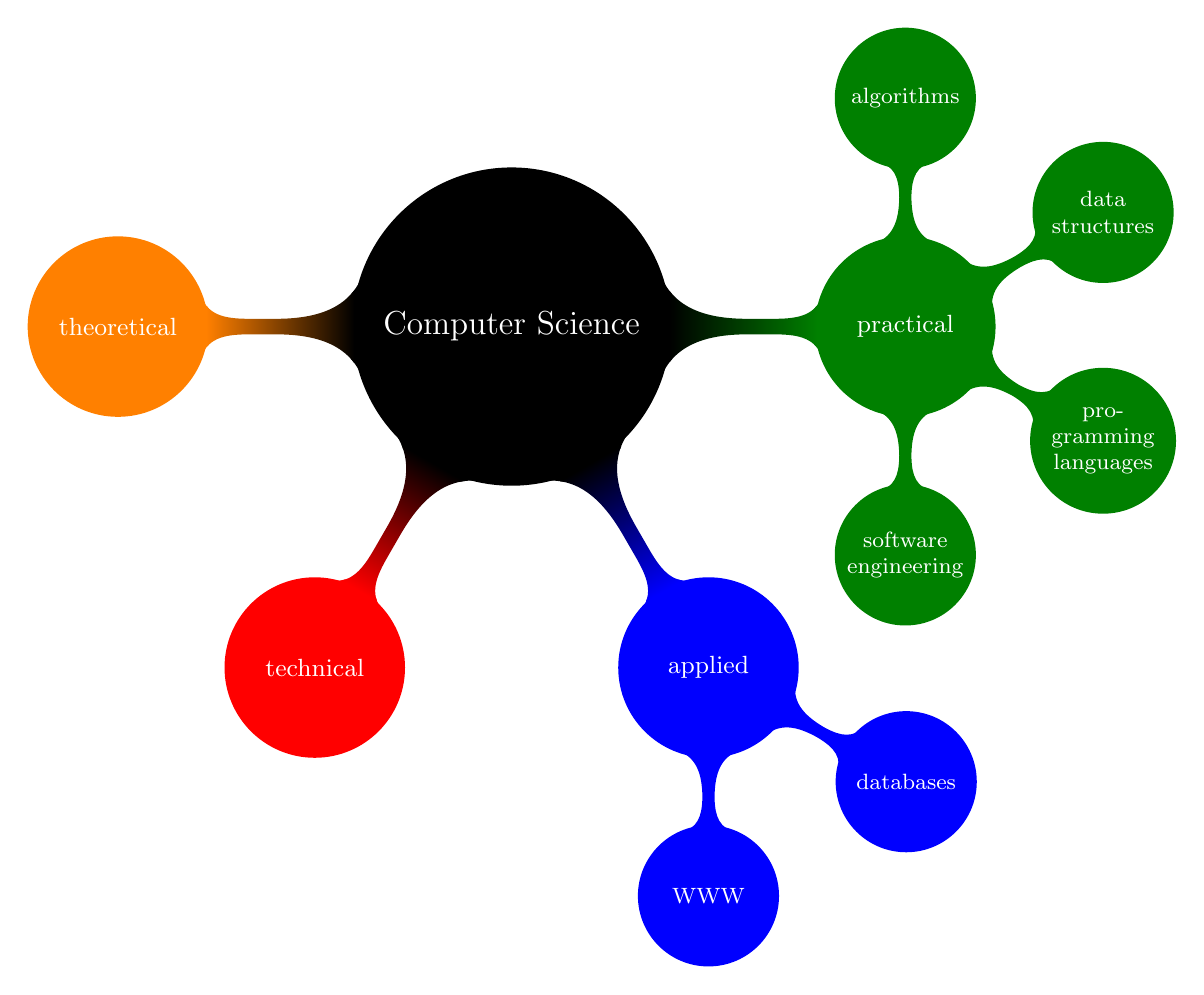
\begin{tikzpicture}
  \path[mindmap,concept color=black,text=white]
    node[concept] {Computer Science}
    [clockwise from=0]
    child[concept color=green!50!black] {
      node[concept] {practical}
      [clockwise from=90]
      child { node[concept] {algorithms} }
      child { node[concept] {data structures} }
      child { node[concept] {pro\-gramming languages} }
      child { node[concept] {software engineer\-ing} }
    }  
    child[concept color=blue] {
      node[concept] {applied}
      [clockwise from=-30]
      child { node[concept] {databases} }
      child { node[concept] {WWW} }
    }
    child[concept color=red] { node[concept] {technical} }
    child[concept color=orange] { node[concept] {theoretical} };
\end{tikzpicture}
\end{document}